\documentclass{article}
\usepackage[T1]{fontenc}
\usepackage{lmodern}
\usepackage{graphicx}
\usepackage{amsmath,amssymb}
\usepackage[a4paper,margin=2cm]{geometry}
\usepackage[absolute,overlay]{textpos}
\setlength{\TPHorizModule}{1mm}
\setlength{\TPVertModule}{1mm}
\usepackage[indonesian]{babel}
\usepackage{hyperref}
\setlength{\emergencystretch}{2em}
% unit: Halaman 56

\begin{document}

% === Halaman 56 (llm) ===

\textbf{Contoh 1:} Misalkan $a = 00001101 = x^3 + x^2 + 1$ dan $b = 00000110 = x^2 + x$

$a$ dan $b \in GF(2^8)$ \quad (dalam notasi Hex, $a = \text{'0D'}$ dan $b = \text{'06'}$)

(i) $a + b = \text{'0D'} + \text{'06'} = (x^3 + x^2 + 1) + (x^2 + x) = x^3 + 2x^2 + x + 1 \pmod{2}$

\vspace{5mm}

\begin{align*}
&= x^3 + 0x^2 + x + 1 \\
&= x^3 + x + 1 = 00001011 = \text{'0B'}
\end{align*}

Dalam representasi biner:

\begin{tabular}{ll}
00001101 \\
\underline{00000110} + \\
00001011 $\rightarrow$ sama dengan hasil operasi XOR
\end{tabular}

\vspace{5mm}

$\therefore a + b = 00001011 = a \text{ XOR } b$

% deskripsi: Teks instruksi berwarna merah yang menjelaskan operasi modulo 2 pada koefisien polinomial: 'Bagi tiap koefisien dengan 2, lalu ambil sisanya'
% bbox normalisasi: [0.5600, 0.2800, 0.7500, 0.3600]
\begin{textblock*}{39.90mm}(117.60mm,83.16mm)
\noindent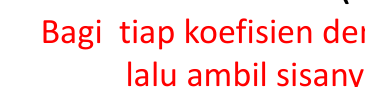
\includegraphics[width=39.90mm,height=23.76mm]{../../images/llm/page_056_img_01.png}%
\end{textblock*}

\end{document}
